\chapter{Design of the vacuum chamber}

This section describes the design of the vacuum vessel, as well as the location and the dimensions of the ports.
It includes our working progress of different vessel designs and the FEM simulations of the different lids.
Also the different ports and feedthroughs are described in detail, for different purposes.

\section{Main recipient}
\label{sec:main_recipient}

The main chamber is a simple cylinder which, including the flange, should have a size, that fits through a regular door ( ca. 200 cm x 90 cm), so a volume of min. 160 cm x 60 cm was chosen for the recipient itself (see \autoref{fig:main}).

\begin{figure}[H]
    \centering
    \begin{subfigure}[b]{0.49\textwidth}
        \centering
        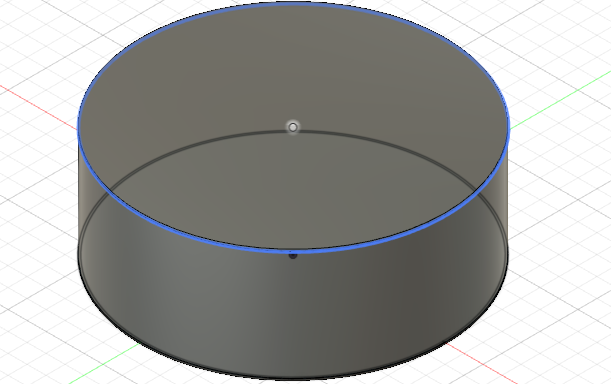
\includegraphics[width=1\textwidth]{sections/imges/vacuum_vessel/Keksdose.PNG}
        \subcaption{Main recipient.}
        \label{fig:main}
    \end{subfigure}
    \hfill
    \begin{subfigure}[b]{0.49\textwidth}
        \centering
        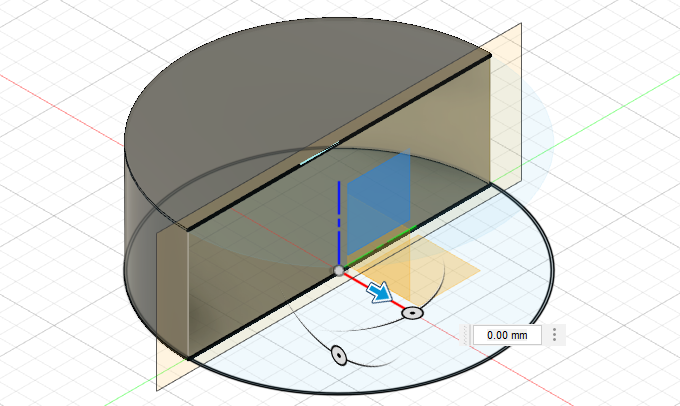
\includegraphics[width=1\textwidth]{sections/imges/vacuum_vessel/Keksdose_Schnitt.PNG}
        \subcaption{Sectional analysis of the main recipient.}
        \label{fig:Schnitt_keks}
    \end{subfigure}
    \caption{Main recipient.}
\end{figure}

The sectional analysis shows that the interior is naturally hollow (see \autoref{fig:Schnitt_keks}), the walls, lid and base are currently 10 mm thick, although depending on the choice of central opening, the lid may be replaced by a large flange/curved top and bottom realizations with and without supporting struts.
Depending on the choice of base on which the vacuum chamber will ultimately stand, consideration should also be given to possible supports for the base and lid to prevent the respective surfaces from buckling.


\subsection{Flanges}

In \autoref{fig:flansch} and \autoref{fig:Schnitt_flange} the raw version of a flange and its sectional analysis is visible.
There is also the possibility to assemble the flanges with the help of various libraries either from readily available parts (McMaster Carr) or to download ready-made flanges (traceparts e.g. registration required).
In both cases, however, it must be known which tasks they need to fulfill.


\begin{figure}[H]
    \centering
    \begin{subfigure}[b]{0.49\textwidth}
        \centering
        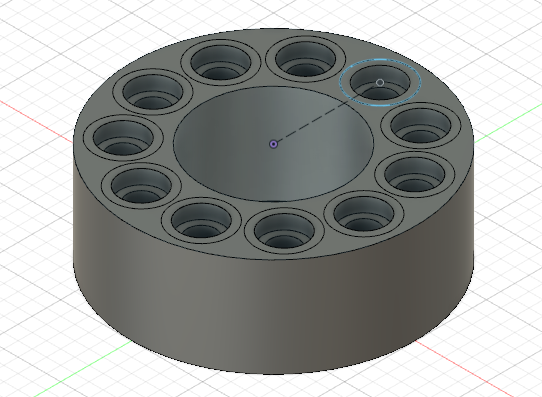
\includegraphics[width=1\textwidth]{sections/imges/vacuum_vessel/Flange.PNG}
        \subcaption{Raw version of a flange}
        \label{fig:flansch}
    \end{subfigure}
    \hfil
    \begin{subfigure}[b]{0.49\textwidth}
        \centering
        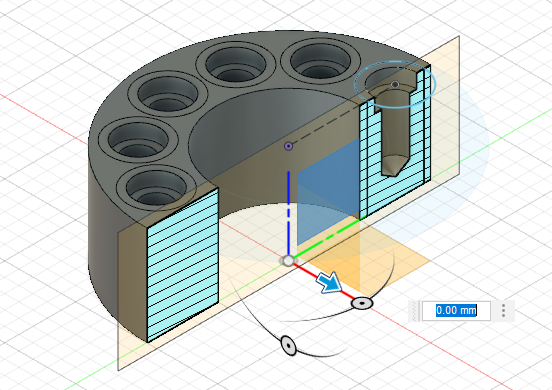
\includegraphics[width=1\textwidth]{sections/imges/vacuum_vessel/Flange_Schnitt.PNG}
        \subcaption{Sectional analysis of the flange.}
        \label{fig:Schnitt_flange}
    \end{subfigure}
    \caption{Flanges.}
    \label{fig:flanges}
\end{figure}

\subsection{Drill holes - options for installing windows and connections}

\begin{figure}[h]
    \centering
    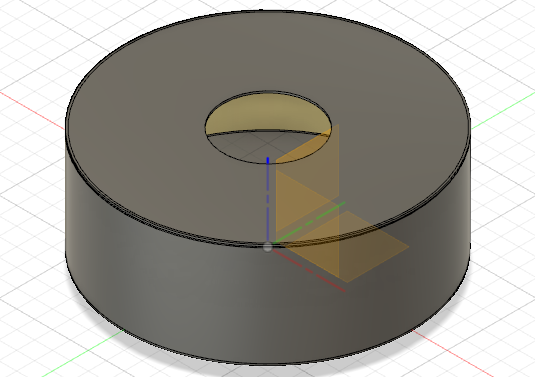
\includegraphics[width=0.55\textwidth]{sections/imges/vacuum_vessel/Bohrung.PNG}
    \caption{Drill hole as a possibility to realize a window in the cover.}
    \label{fig:Bohrung}
\end{figure}

With the help of the drilling tool, openings can be made in the existing solid body relatively easily and without complications, but once the hole has been made at a certain point, it can no longer be moved.
However, it is possible to go back in time to the point at which the hole was drilled and drill it again (see \autoref{fig:Bohrung}).

\subsection{FEM simulations for different lid designs}

The FEM simulations have shown that a domed lid on a cylindrical shell delivers the best results for stability against bending.
The deformation due to the vacuum pressure is in this case max. $16\ \si{\micro\meter}$.
The wall thickness is still $10\ \si{\milli\meter}$.
The combination with a domed base is also possible, but involves the same difficulties as the domed lid (higher production complexity, potential customization, higher costs and special chamber support required for curved bottom).
In the case of a curved lid, a thickness of $2\ \si{\centi\meter}$ is sufficient.
In addition, it would have to be considered how the entire chamber is held/stabilized and how/where the flanges of the pumps can then be attached.
The inside diameter of the chamber is $160\ \si{\centi\meter}$ and the inner height $65\ \si{\centi\meter}$.

\begin{figure}[H]
    \centering
    \begin{subfigure}[b]{0.3\textwidth}
        \centering
        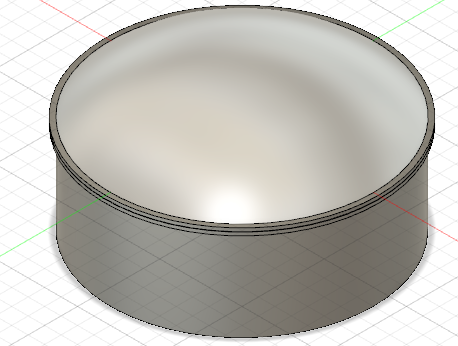
\includegraphics[width=1\textwidth]{sections/imges/vacuum_vessel/Kekskochtopf.PNG}
        \subcaption{}
        \label{fig:Kekskochtopf}
    \end{subfigure}
    \hfil
    \begin{subfigure}[b]{0.59\textwidth}
        \centering
        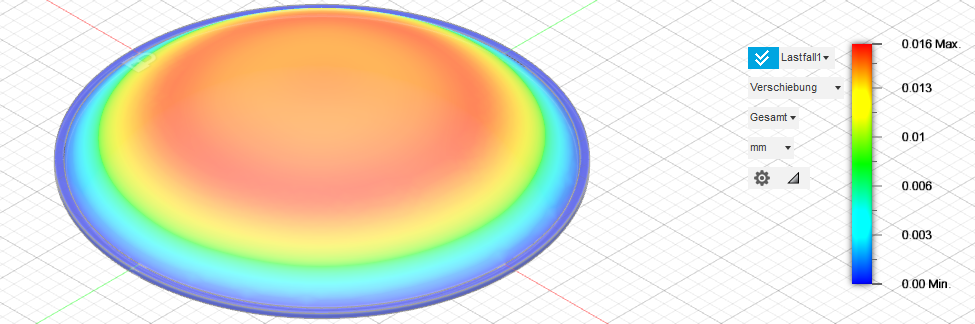
\includegraphics[width=1\textwidth]{sections/imges/vacuum_vessel/Kekskochtopf_Simu.PNG}
        \subcaption{Domed lid: max. displacement at $p = 1$ bar: $16\ \si{\micro\meter}$}
        \label{fig:Kekskochtopf_FEM}
    \end{subfigure}
    \caption{Vacuum vessel with curved lid.}
    \label{fig:Kekskochtopf_all}
\end{figure}

The second variant would be a flat lid and base with struts.
In this case, the displacements as a result of the deformations would be in the region of $100\ \si{\micro\meter}$ , but production would probably be cheaper and simpler.
One disadvantage of this design is that the large struts mean that there is less space available for potential flanges.

\begin{figure}[H]
    \centering
    \begin{subfigure}[b]{0.3\textwidth}
        \centering
        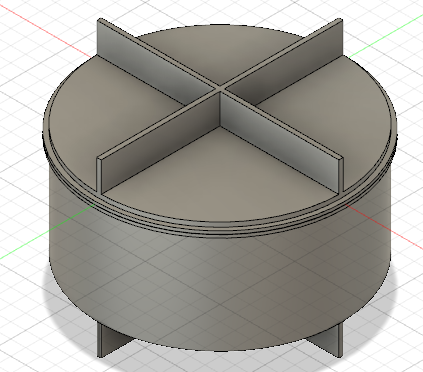
\includegraphics[width=1\textwidth]{sections/imges/vacuum_vessel/Keksdose_Streben.PNG}
        \subcaption{}
        \label{fig:Strebendose}
    \end{subfigure}
    \hfil
    \begin{subfigure}[b]{0.59\textwidth}
        \centering
        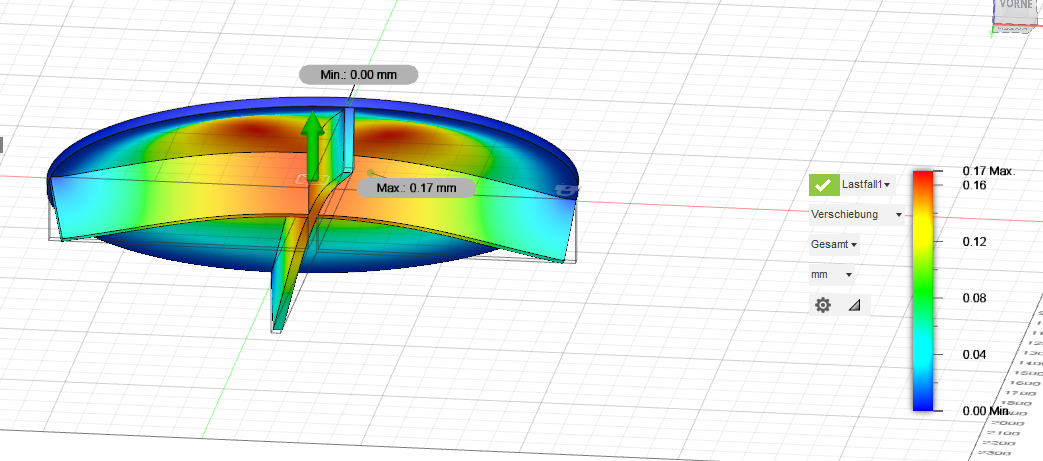
\includegraphics[width=1\textwidth]{sections/imges/vacuum_vessel/Simulation_palatschinkendeckel_mit_Streben_30.PNG}
        \subcaption{Lid-simulation: max. displacement at $p = 1$ bar: $100\ \si{\micro\meter}$}
        \label{fig:Strebendose_FEM}
    \end{subfigure}
    \caption{Vacuum vessel with struts.}
    \label{fig:Strebendose_all}
\end{figure}

The FEM simulation of a simple cover leads to a displacement of more than $ 1\ \si{\milli\meter}$, which is too much.
The bottom plate of the chamber was chosen to be flat, with a thickness of $50\ \si{\milli\meter}$.
This also makes it easier to attach the coils inside of the chamber, as in the case of a flat bottom, additional brackets and stabilizers for the coils could be dispensed with, as they would stand more or less on the bottom.
This setup is shown in \autoref{fig:Dose_all}.

\begin{figure}[H]
    \centering
    \begin{subfigure}[b]{0.4\textwidth}
        \centering
        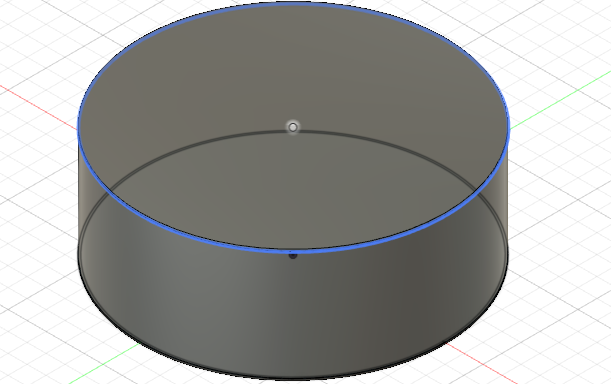
\includegraphics[width=1\textwidth]{sections/imges/vacuum_vessel/Keksdose.PNG}
        \subcaption{}
        \label{fig:Dose}
    \end{subfigure}
    \hfill
    \begin{subfigure}[b]{0.49\textwidth}
        \centering
        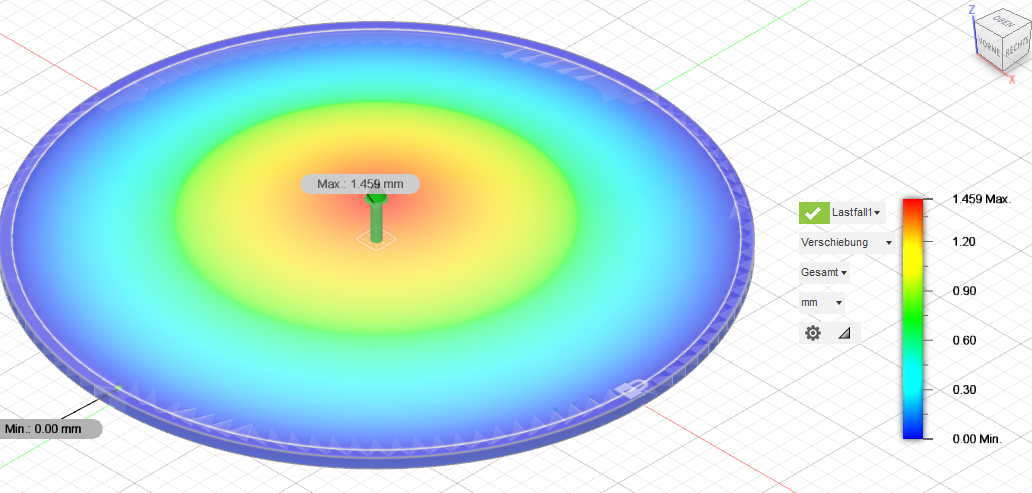
\includegraphics[width=1\textwidth]{sections/imges/vacuum_vessel/Simulation_palatschinkendeckel.PNG}
        \subcaption{Lid-simulation: max. displacement at $p = 1$ bar: $>1\ \si{\milli\meter}$}
        \label{fig:Dose_FEM}
    \end{subfigure}
    \caption{Vacuum vessel.}
    \label{fig:Dose_all}
\end{figure}


% A hot cathode tube can be used as a pressure gauge in the HV, as it does not require a magnetic field.
% Either a Pirani or a piezoresistive pressure transducer is suitable for the fore-vacuum.

% \celena{remove when included in text}
% \todo{What is which this paragraph?}


\subsection{Finished design for the time being:}
The various flanges are connected to the vacuum chamber step by step, starting with those of the vacuum team, as we are already familiar with them.
In the meantime, some questions have arisen whose answers can be found below:

\begin{itemize}
    \item A mirror can be moved in a vacuum chamber using piezo crystals, which should be accurate enough for the application of an interferometer.
    \item The position of the TMP should be chosen so that another one can be added easily and without complications. (Therefore, perhaps simply add a second flange).
    \item An extremely rough inner surface of the vacuum chamber would be bad, but does not really occur with stainless steel. If necessary, it can always be reground.
    \item The cleanliness of a vacuum chamber is very important. The best way to clean it is with a cleaning sponge (green side) and Atta (scouring agent). If necessary, follow up with isopropanol.
\end{itemize}

The shape of the vacuum chamber chosen for the time being is as visible in \autoref{fig:Kammer_all}.
The decision was made in favor of a curved cover and base, as this provides enough space for the coils and also best counteracts the deflection caused by the pressure difference (see \autoref{fig:Kekskochtopf_FEM}, the calculation of the FEM simulation results in the lowest displacement for this).

As the base of this model is also curved, as can be seen, a supporting structure is required.
Possible implementations are shown at \autoref{fig:Halterung}.
The supporting structure are welded on steel lips on the side of the chamber.
This lips are than placed onto steel frame outside of the chamber.
Depending on how well this idea fits in with other realizations of the other four groups, it will also be added to the Fusion360 model.


\begin{figure}[H]
    \centering
    \begin{subfigure}[b]{0.4\textwidth}
        \centering
        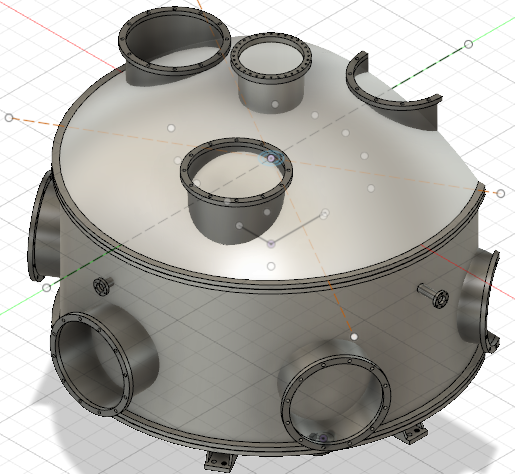
\includegraphics[width=1\textwidth]{sections/imges/vacuum_vessel/Vakuumkammer_final.PNG}
        \subcaption{Final version of the vacuum chamber.}
        \label{fig:Kammer}
    \end{subfigure}
    \hfill
    \begin{subfigure}[b]{0.4\textwidth}
        \centering
        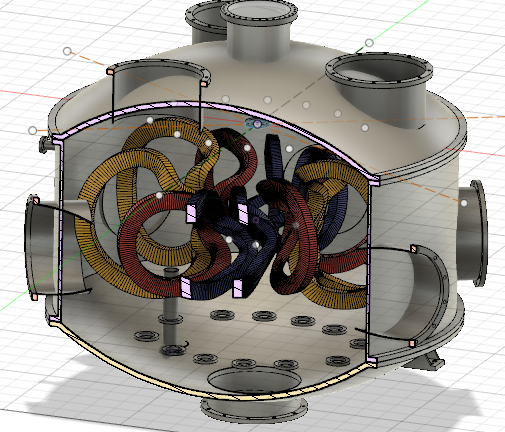
\includegraphics[width=1\textwidth]{sections/imges/vacuum_vessel/Vakuumkammer_final_Schnitt.PNG}
        \subcaption{Sectional analysis of the chamber: The flanges for the coil connections facing inwards are visible on the inside. }
        \label{fig:Kammer_Schnitt}
    \end{subfigure}
    \caption{Views of the currently completed vacuum chamber}
    \label{fig:Kammer_all}
\end{figure}

\begin{figure}[H]
    \centering
    \begin{subfigure}[b]{0.3\textwidth}
        \centering
        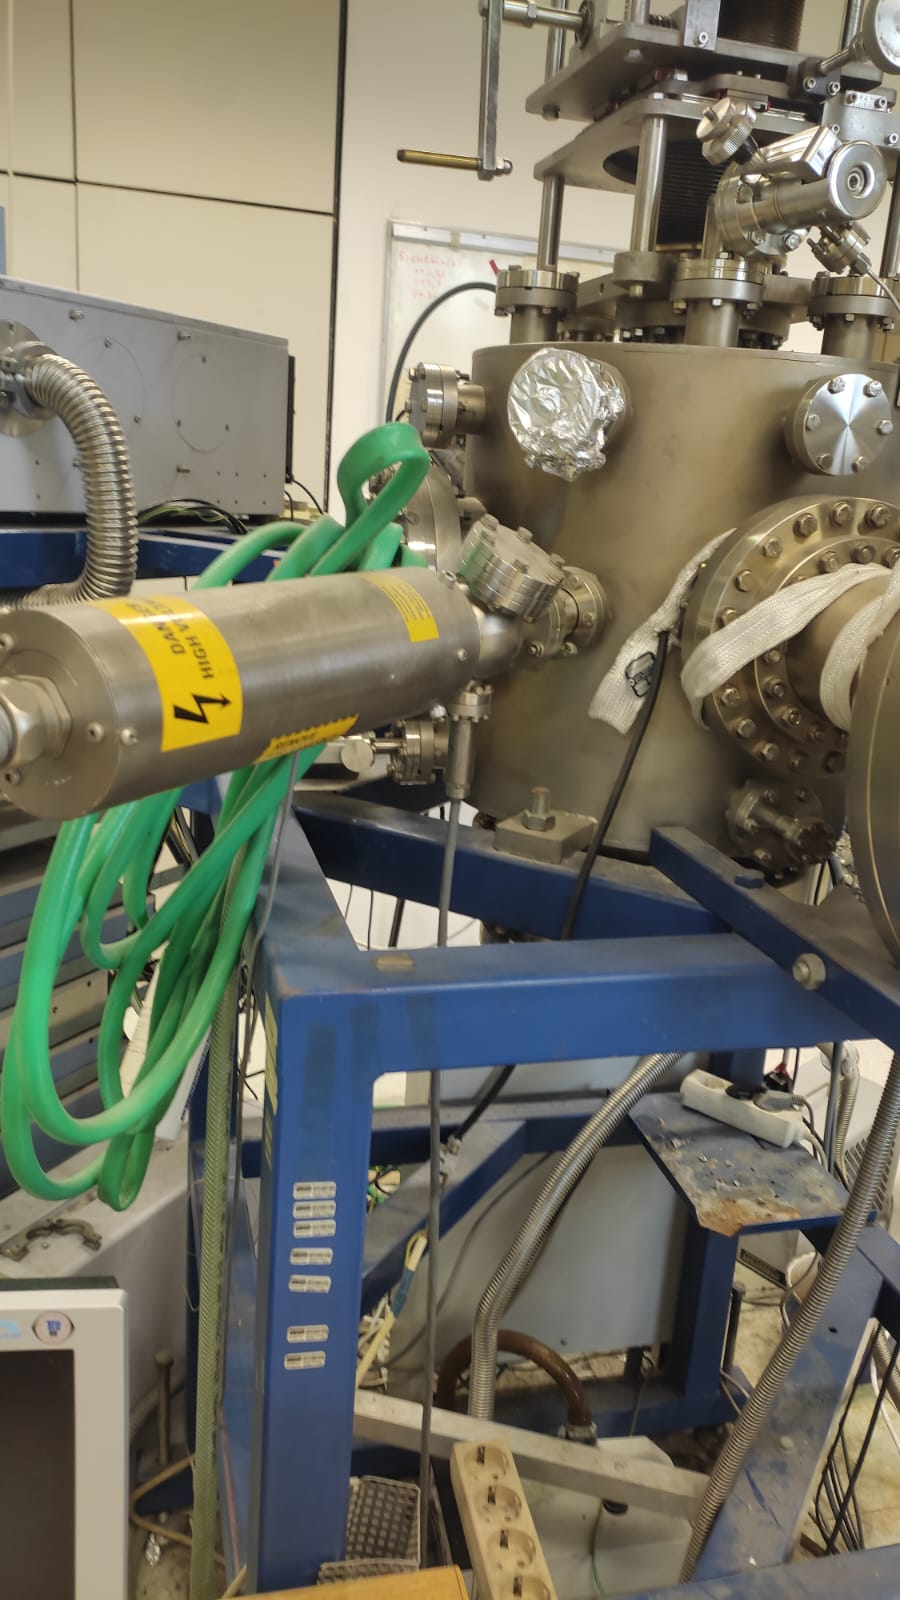
\includegraphics[width=1\textwidth]{sections/imges/vacuum_vessel/Halterung1.jpeg}
        \subcaption{Option to mount the vacuum chamber for the support function.}
        \label{fig:Halterung1}
    \end{subfigure}
    \begin{subfigure}[b]{0.3\textwidth}
        \centering
        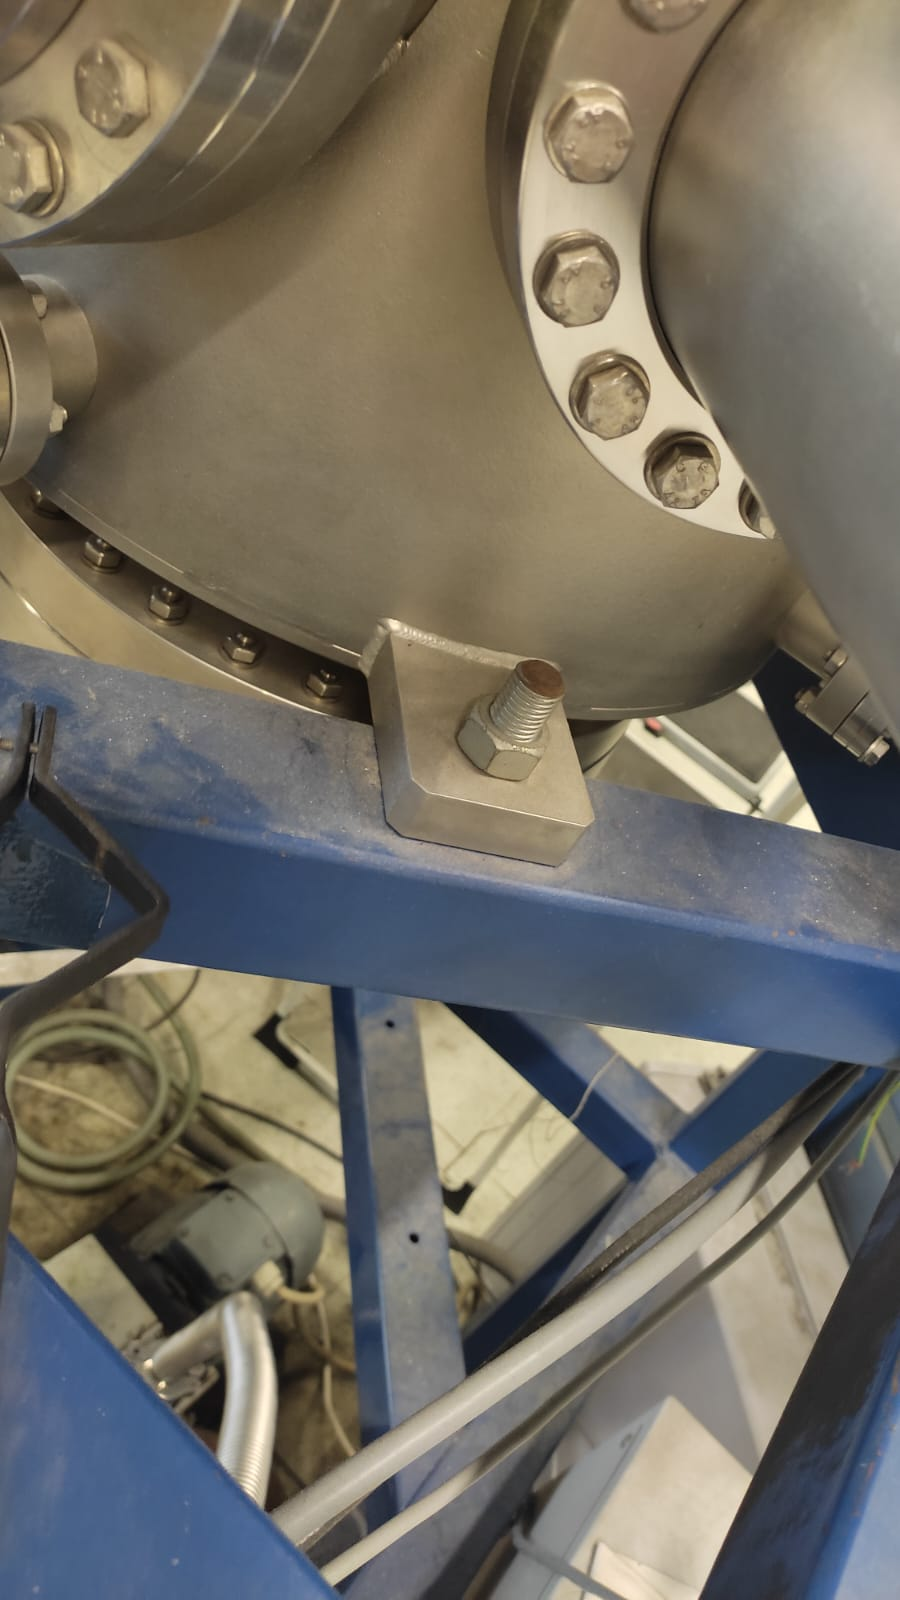
\includegraphics[width=1\textwidth]{sections/imges/vacuum_vessel/Halterung2.jpeg}
        \subcaption{Stabilizing feet for attaching the chamber to the support frame.}
        \label{fig:Halterung2}
    \end{subfigure}
    \caption{Possibility of stabilizing and fastening the vacuum chamber so that flange connections are possible on the floor and are freely accessible.}
    \label{fig:Halterung}
\end{figure}

The mounting and the positioning of the coils inside the chamber is in the responsibility of the coil team.
One need to mention that the coils should be able to be fine adjusted from the outside when the chamber is closed and evacuated.
For this purpose, the coils should be mounted on ballows, which allows the movement of the coils.


\section{Ports and feedthrough}

\subsection{(Double) o-ring gasket}

To include different vacuum equipment, the components need to have a sealing surface, at which the equipment can be pressed together.
A filled with elastic or plastic sealant is used due to the deviation of the ideal shape in order to make a vacuum tight connection. \cite{Wutz2000}

For the large lid a double o-ring can be used to reduce the pressure difference between the inside and the outside of the chamber.
This large diamantions of the chamber make the gasket of the lid more difficult.
Fortunately, the chamber is not under high pressure, so a Viton\textsuperscript{TM} seal can be used.


\subsection{Copper gasket}
For the smaller flanges especially when the temperature are high, a copper seal is used.
The high temperature can be caused by the back out of the chamber to get a better vacuum, which out water.
Thus for temperatures above $300\si{\degreeCelsius}$ a copper gasket is used, which does not outgas.
For this a CF-flange is used, which is made of stainless special steel of high hardness
As gasket a oxygen free copper gasket (OFHC) is used.
The copper should have a hight ductility, in order to make a good seal.
This sustains temperatures up to $450\si{\degreeCelsius}$.
One downside of the copper gasket is that it can only be use once, because it deforms.
Thus it should be used for flanges which are not opened often \cite{Wutz2000}.




\subsection{Gas injection ports}

To allow a controlled introduction of the gas into the vacuum chamber dosing valves are used as gas inlet ports.
They are used to introduce precisely defined gas flows.
The dosing valves, also known as precision valves, operate based on the principle of a needle valve and allow for a reproducible adjustment of the valve opening using a micrometer screw.
The opening gap of the valve determines the gas inlet rate and measures the conductance.
For commercially used dosing valves the gas inlet rates ranges from $10^{-6}~\si{\cubic\centi\meter\per\second}$ to $10^{3}~\si{\cubic\centi\meter\per\second}$.

The positions of the gas inlet ports are not critical.
They mainly should be positioned in such a way that the gas is evenly distributed in the chamber and efficient pumping is enabled.
Since the turbomolecular pump will be positioned at the bottom of the vacuum vessel, the gas inlet ports could be positioned at the top or on the sides of the vessel \cite{Wutz2000}.

\subsection{Ventilation valves}
Ventilation valves, also known as vacuum relief valves, are used to control the pressure within the system.
Generally, you want to place the ventilation valves in a location where one can effectively regulate the pressure throughout the chamber.
An example valve from the company Pfeiffer is shown in \autoref{fig:ventilation-valve}.
This valve is made of stainless steel and is manually actuated.
It uses a DN 10 ISO-KF flange connection, which is a standard connection for vacuum applications.

\begin{figure}[H]
    \centering
    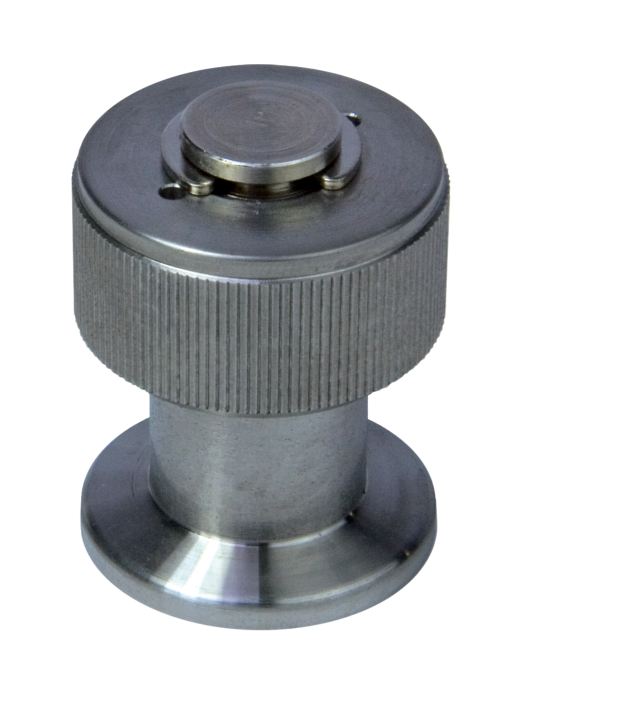
\includegraphics[width=0.3\textwidth]{sections/imges/ports/venting_valve.png}
    \caption{Example ventilation valve from Pfeiffer with an DN 10 ISO-Kf fange \cite{pfeiffer_venting_valve}.}
    \label{fig:ventilation-valve}
\end{figure}


\subsection{Windows}
Regarding windows one would have several options to choose from.
The simplest solution would be \textbf{acrylic blind fanges} but they might not provide the necessary tightness or optical quality.
Since these windows form a part of the vessel they replicate some essential functions of the wall.
They need to be leak proof to maintain the vessel's vacuum, and they must ensure nuclear confinement.
As a result, \textbf{glass windows}, some of which are plane-ground, are typically preferred.
\textbf{Melted-in panes} are the only ones that can achieve extreme tightness and heat-ability.
To maximize the viewing angle, the glass pane should ideally be positioned in the plane of the vessel wall.
These windows can be produced with diameters up to 150 mm as standard, and the glass surface can be coated for anti-reflection or to prevent static charges. UHV viewing glasses, which need to withstand high energy doses (typically 10$^6$ J $\cdot$ kg$^{-1}$ per year), must be radiation-resistant.
For this purpose, either radiation-resistant types of glass or \textbf{sapphire windows} are used.
The material is very resistant and can withstand high energy doses. It is more expensive than glass, but it offers excellent optical properties and high resistance to scratches and abrasion.
Commonly, sapphire discs (25 mm and 50 mm) are metallized using the molybdenum-manganese method (refer to section 14.1.4) and are vacuum-sealed to a thermally adapted Ni-Fe pipe piece.\cite{Wutz2000} We decided to use \textbf{quartz glass}, which is also an option due to its resistance to extremly high temperatures and to radiation and its excellent transparency in UV and IR range, which can be usefull for diagnostic purpose, as it allows a clear view of the plasma.
Additionally it as a very low outgassing rate, therefore it won't disturb the vacuum in the Stellarator.
An example window from Pfeiffer is shown in \autoref{fig:window}.
This window is made of stainless steel and fused silica and uses a DN 100 CF flange connection.



\begin{figure}[H]
    \centering
    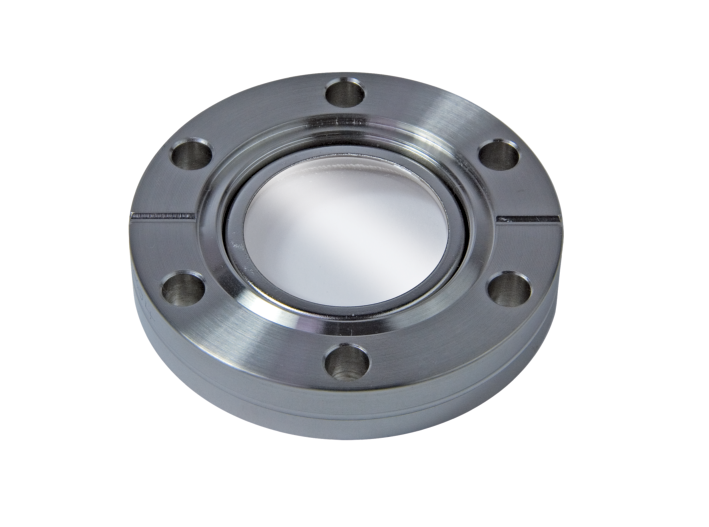
\includegraphics[width=0.3\textwidth]{sections/imges/ports/vacuum_window.png}
    \caption{Example Window from Pfeiffer with an DN 100 CF flange \cite{pfeiffer_window}.}
    \label{fig:window}
\end{figure}



\subsection{Sealings}
For moving parts flexible spring bodies are preferably used as seals.
These components can be heated higher than the other penetrations, are absolutely tight and allow a sufficient number of switching operations with the correct design.
The length of these elements is determined by the required stroke. Therefore, valves with large nominal sizes are equipped with a vacuum translation to save space.
In general, the sealing of the valve seat is done with a ring made of Perbunan or Viton.
The tightness is sufficient for most applications.
The valves can be heated up to about 150 °C when using Viton.
At a working pressure below about 10$^{-7}$ mbar, the gas release of the elastomers begins to interfere.
Therefore, metal seals are used for flanges and housings.
The O-ring on the valve seat is often retained even at lower pressures, as valves with all-metal sealing on the valve seat require very high forces and are particularly complex, especially in the larger diameter range \cite{Wutz2000}.

\subsection{Current feedthrough}

As the vacuum chamber is made out of metal, the current feedthrough must be isolated to the chamber wall.
For this usually plastics, glass or ceramics are used.
Due to the heat expansion the connection between the chamber and the insulator must be done properly, as it causes a lot of stress on the insulator \cite{Wutz2000}.

The different insulators have different temperature resistance.
For low temperatures, up to $\approx 80\si{\degreeCelsius}$, plastics can be used.
For higher temperatures glass or ceramics are used.
Here, one must be careful that the material of the chamber and the insulator have a similar heat expansion coefficient.
Otherwise it can come to leakages or failure of the insulator \cite{Wutz2000}.
A plastic insulator is shown in \autoref{fig:plastic_insulator} and a ceramic insulator in \autoref{fig:ceramic_insulator}.


\begin{figure}[H]
    \centering
    \begin{subfigure}[t]{0.49\textwidth}
        \centering
        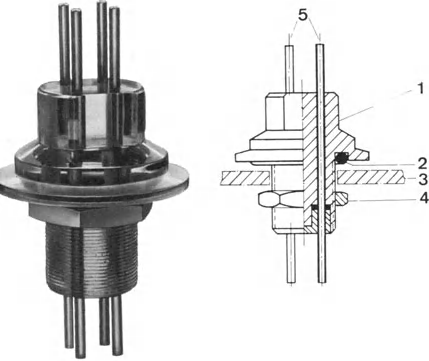
\includegraphics[width=1\textwidth]{sections/imges/seals/plastic_insulator.png}
        \subcaption{Plastic insulator with multi current feedthrough. 1 Plastic body, designed as a small flange; 2 Rubber-elastic sealing ring; 3 Wall with hole; 4 Fastening nut; 5 Metal rods or pipes.}
        \label{fig:plastic_insulator}
    \end{subfigure}
    \hfill
    \begin{subfigure}[t]{0.49\textwidth}
        \centering
        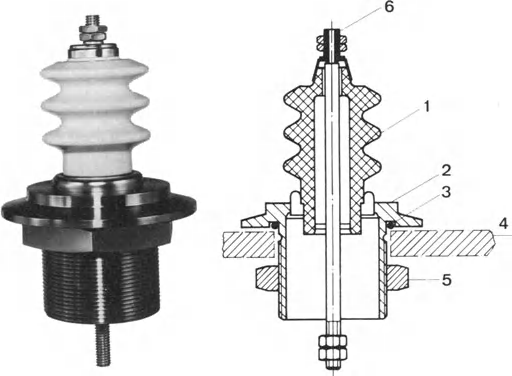
\includegraphics[width=1\textwidth]{sections/imges/seals/ceramic_insulator.png}
        \subcaption{High-voltage bushing insulated with ceramic (test voltage $25~\si{\kilo\volt}$). 1 Ceramic body; 2 Small flange with pipe connection; 3 Rubber-elastic seal; 4 Wall with hole; 5 Fastening nut; 6 Metal rod or metal pipe.}
        \label{fig:ceramic_insulator}
    \end{subfigure}
    \caption{Current feedthrough with (a) plastic insulator and (b) ceramic insulator \cite{Wutz2000}.}
\end{figure}

It should be noted that the dielectric strength is greatest for hight pressure ($\approx 1~\si{\bar}$) and very low pressers (HV to UHV).
This holdes true especially for high voltage ($\approx 300~\si{\volt}$).
For pressures in between the dielectric strength is reduced, thus a electrical breakdown or a gas discharge can occur.
Therefore, during evacuation and ventilation of the chamber, the voltage should be switched off \cite{Wutz2000}.

\subsection{Coaxial feedthrough}

\begin{figure}[H]
    \centering
    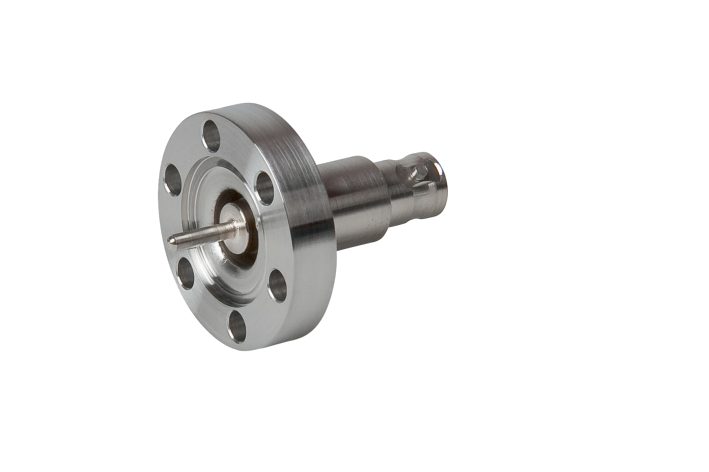
\includegraphics[width=0.5\textwidth]{sections/imges/ports/coaxial_feedthrough_pfeiffer.png}
    \caption{Example for a coaxial feedthrough from Pfeiffer \cite{pfeiffer_coaxial}.}
    \label{fig:coaxial_feedthrough}
\end{figure}

The Grounded Shield-coaxial feedthrough features shielding potential located on the flange or welding lip.
This ensures effective shielding by connecting the shield to the flange.
The current rating applies per pin, and the flange material is stainless steel.
The connector is designed for atmospheric conditions ranging from $\SI{-65}{\degreeCelsius}$ to $\SI{165}{\degreeCelsius}$.
The specified voltages and currents are based on specific environmental conditions, including room temperature, dry external air, and internal vacuum of less than $\SI{e-4}{\hecto\pascal}$ \cite{pfeiffer_coaxial}.


\subsection{Cooling liquid feedthrough}
When the temperature changes a lot of mechanical stress can be put on weldes and solder joints. For this case the connection between the flange and the pipe is reduced by a long and thin-walled transition piece (e.g.: a metal hose of chrome-nickel steel).
The flange then retains its normal temperature, and the flowing medium is only slightly affected \cite{Wutz2000}.

\section{Manipulators (Mechanical feedthroughs)}


Mechanical manipulators, also known as mechanical feedthroughs, are used to transfer movements from outside a vacuum chamber into the vacuum.
They typically consist of a force-transmitting element (shaft), a seal, and a flange. These manipulators are categorized into three groups: those with dynamic seals, flexible elements, and magnetic force coupling.
Manipulators with flexible elements, such as membrane or bellows, enable many precise movement types and are characterized by their lack of dynamic leakage rate. The lifespan is determined by the sizing and stress of the bellows.
Manipulators with dynamic seals, such as O-ring-sealed and magnetofluid-sealed manipulators, exhibit a dynamic leakage rate between stationary and moving elements, which is typically greater than the static leakage rate. O-ring-sealed manipulators undergo continuous seal wear \cite{jousten_handbuch_2018}.




\subsection{Bellows}
\
\begin{figure}[H]
    \centering
    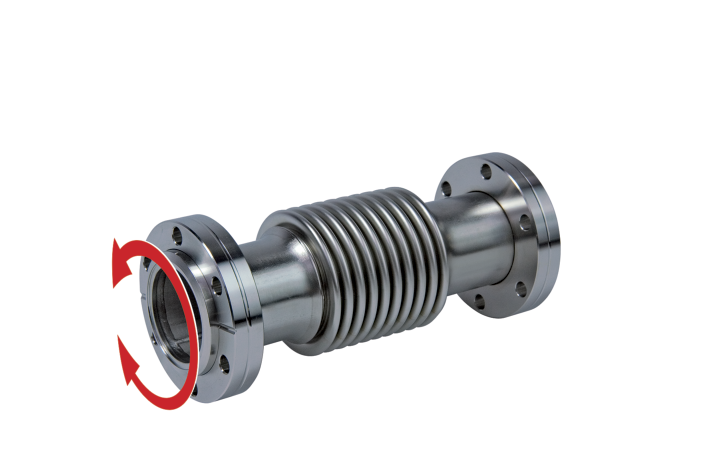
\includegraphics[width=0.5\textwidth]{sections/imges/ports/bellows.png}
    \caption{Example for a vacuum bellow \cite{pfeiffer_bellows}.}
    \label{fig:pfeiffer_bellow}
\end{figure}

\autoref{fig:pfeiffer_bellow} features a rotatable flange on one end and a fixed flange on the other end, allowing for flexibility in alignment and vibration resistance \cite{pfeiffer_bellows}.
Bellows are used in feedthroughs with flexible elements, allowing for a wide range of precise movements.
The lifespan of bellows feedthroughs is determined by the dimensioning and stress on the bellows, making proper design crucial for longevity \cite{jousten_handbuch_2018}.

\subsection{Manipulator for Langmuir probe}

As a manipulator for Langimur probe one could use mechanical feedthroughs with flexible elements. These enable precise types of movement and are characterized by a low dynamic leakage rate \cite{jousten_handbuch_2018}.

\subsection{Pieco motor for the interferometer mirror}

One could use a vacuum-compatible Piezo linear motor actuator with Teflon-coated leads for seamless integration with vacuum-chamber feedthroughs.
To ensure precise motion control and stability one could also consider the use of a closed-loop Picomotor controller and driver.
This configuration, along with suitable sensor signal plug-in cards, provides the sub-nanometer resolution necessary for precise positioning and manipulation of the interferometer mirror within the vacuum chamber \cite{pie, piez0}.


\begin{figure}[H]
    \centering
    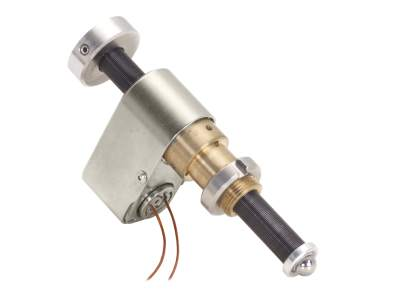
\includegraphics[width=0.4\textwidth]{sections/imges/piezo.jpg}
    \caption{Example for a vacuum compatible picomotor Piezo linear actuators \cite{pie}.}
    \label{fig:pie}
\end{figure}




\section{Overview of the ports of each team}

\subsection{Vacuum - Team}

\begin{table}[H]
    \centering
    \caption{Overview of the ports from the \textbf{vacuum team}.}
    \begin{tabular}{>{\raggedright\arraybackslash}p{2cm} >{\raggedright\arraybackslash}p{3cm} >{\raggedright\arraybackslash}p{3.5cm} >{\raggedright\arraybackslash}p{2cm} >{\raggedright\arraybackslash}p{3.5cm}}
        \toprule
        \textbf{Port}   & \textbf{Propose}               & \textbf{Location}  & \textbf{Type} & \textbf{Flange/Size}          \\
        \midrule
        Port 1          & Pirani/Bayard-Alpert manometer & outside of chamber &               & DN 40 CF-R                    \\
        Port 2          & Quadrupole mass spectrometer   & outside of chamber &               & DN 40 CF-F                    \\
        \midrule
        Port 3          & Turbo molecular pump (TMP)     & bottom             &               & DN 320 ISO-F                  \\
        Port 4          & Routing pump                   &                    &               & DN 40|50 ISO KF               \\
        \midrule
        Port 5          & Domed lid                      & top                &               & $d = 1600\ \si{\milli\meter}$ \\
        Port 6          & Domed bottom                   & bottom             &               & $d = 1600\ \si{\milli\meter}$ \\
        \midrule
        All other ports & any use                        & side and bottom    &               & DN 320 ISO-F                  \\
        \bottomrule
    \end{tabular}
    \label{tab:vacuum_ports}
\end{table}



For the sake of simplicity, all flange connections were chosen to have the same size.
Only the connections for the Pirani-Bayard-Alpert pressure measurement and the quadrupole spectrometer were chosen differently, as little previous knowledge of specific flange sizes was known.
The universal fange connections chosen for the versatile connection is the same flange used as for the TMP (cf. \autoref{tab:vacuum_ports}).
This flange size was chosen because if a second TMP is needed, it can be easily added to the chamber using a knee.
Also the relative large size of the flange allows to connect other flanges to it using adapters.

The ports for the \textbf{pumps}, especially the TMP, are planned to be located at the bottom of the chamber.
As for our purpose only one TMP will be used, only one port is needed.
Although, one has to keep in mind that it could makes sense to add a second port for a second TMP at the bottom of the chamber, but only if there is enough space available.
However, all the ports are added in such a way that there is enough space for the feet of the vacuum chamber, which carry the entire weight.
Furthermore, there must be enough space under the chamber so that the length of the TMP is sufficient.
The port of the roughing pump does not need to be added to the vessel itself, because it usually can be connected directly to the to TMP.

The location of the flange for the \textbf{pressure measurement} is not critical.
It can be added anywhere to the chamber.
One might chose the exact location when the other port locations are batter known.
A hot cathode tube can be used as a pressure gauge in the HV, as it does not require a magnetic field.
Either a Pirani or a piezoresistive pressure transducer is suitable for the vacuum.
Furthermore in \autoref{sec:pressure_measurement}.

For the residual \textbf{gas analysis} one can use a quadrupole mass spectrometer.
This allows to measure the composition of the gas in the chamber.
This might be useful to check if the gas which was put into the chamber was the correct one.
Additionally, it helps to detect leaks in the chamber.
The position of the flange for the mass spectrometer is not critical.
It can be added anywhere to the chamber.
However, it is not necessary for leak detection to use a mass spectrometer attached the chamber, as there are different methods to do so.
But it make sens to include a flange for future use.

Finally, it should be mentioned that also gas inlets must be added to the chamber.
They will allow a controlled introduction of the gas into the chamber.
The position of these ports can be located anywhere on the chamber and it makes sens to include it last, as they do not take up much space.
Thus, two or three ports can be added if necessary.


\subsection{Coil - Team}
\begin{table}[H]
    \centering
    \caption{Overview of the ports from the \textbf{coil team}.}
    \begin{tabular}{>{\raggedright\arraybackslash}p{2cm} >{\raggedright\arraybackslash}p{3cm} >{\raggedright\arraybackslash}p{3.5cm} >{\raggedright\arraybackslash}p{3.5cm} >{\raggedright\arraybackslash}p{2cm}}
        \toprule
        \textbf{Port} & \textbf{Purpose} & \textbf{Location}                              & \textbf{Type}       & \textbf{Flange/Size} \\
        \midrule
        Port         &    coil connection         & in vicinity of actual coil position (12 coils) &  - &  DN 63 ISO KF  \\
        \bottomrule
    \end{tabular}
\end{table}


The 12 coils are connected to the vacuum chamber by using a DN 63 ISO KF flange.
Each coil itself is included in a singe stainless steel casing, which allows the operation of the coils in atmospheric conditions, while the chamber is evacuated.
This setup excludes the coils from the vacuum, which makes it easier to run the reactor, as the cooling and power supply of the coils gets easier.

The exact positioning and mounting of the coils is in the responsibility of the coil team.



\subsection{Design - Team}
%\begin{table}[H]
    \centering
    \caption{Overview of the ports from the \textbf{design team}.}
    \begin{tabular}{>{\raggedright\arraybackslash}p{2cm} >{\raggedright\arraybackslash}p{3cm} >{\raggedright\arraybackslash}p{3.5cm} >{\raggedright\arraybackslash}p{3.5cm} >{\raggedright\arraybackslash}p{2cm}}
        \toprule
        \textbf{Port} & \textbf{Purpose} & \textbf{Location} & \textbf{Type} & \textbf{Flange/Size} \\
        \midrule
        Port 1        & Waveguide        & ?                 &               & UDR26                \\
        Port 2        & Window           & ?                 & round         &                      \\
        \bottomrule
    \end{tabular}
\end{table}

Unfortunately we did not got exact specifications nor exact definitions of their ports or locations.

\subsection{Diagnostic - Team}
\begin{table}[H]
    \centering
    \caption{Overview of the ports from the \textbf{diagnostic team}.}
    \begin{tabular}{>{\raggedright\arraybackslash}p{2cm} >{\raggedright\arraybackslash}p{3cm} >{\raggedright\arraybackslash}p{3.5cm} >{\raggedright\arraybackslash}p{3.5cm} >{\raggedright\arraybackslash}p{2cm}}
        \toprule
        \textbf{Port} & \textbf{Purpose}  & \textbf{Location}                 & \textbf{Type} & \textbf{Flange/Size}                                              \\
        \midrule
        Port 1        & electron gun   & Side (between two coils)                    &               & DN100 CF                                                                  \\
        Port 2        & Window            & Side ($75\si{\degree}$ to Port 1) &               & DN400 ISO-F                                              \\
        \midrule
        Port 3        & Langmuir probe / fluorescence rod    & Side (between two coils)                     &               & DN400 ISO-F \\
        Port 4 - 6    & Interferometer    & bottom next to the vacuum pump flange                                 &              & DN320 ISO-K                                                                 \\
        Port 7        & Rogowski coil     &$120~\si{\degree}$ to each component(two diamagnetic loops and one Rogowski coil)                                   &     & DN25-KF                                                                  \\
        Port 8 - 9    & Diamagnetic loops &$120~\si{\degree}$ to each component(two diamagnetic loops and one Rogowski coil)                                   &     &    DN25-KF                                                               \\

        \bottomrule
    \end{tabular}
\end{table}



Port 1 is the \emph{Fluorescent rod}, its purpose is to magnetic field in the vacuum chamber.
It has to be removed when the heating is started, thus it \textbf{must} be moveable.
The location of this probe should be radial to the center of the chamber and the coils, respectively.
An example of such a fluorescent rod is shown in \autoref{fig:fluorescent_rod}.

\begin{figure}[H]
    \centering
    \begin{subfigure}[b]{1\textwidth}
        \centering
        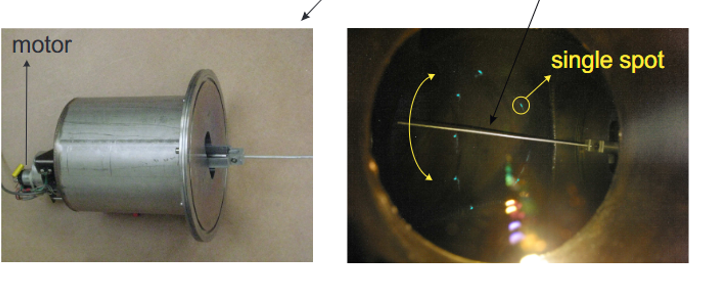
\includegraphics[width=0.7\textwidth]{sections/imges/ports/fluorescent_rod.png}
        \subcaption{Fluorescent rod in the vacuum chamber.}
        \label{fig:fluorescent_rod}
    \end{subfigure}
    \hfill
    \begin{subfigure}[b]{1\textwidth}
        \centering
        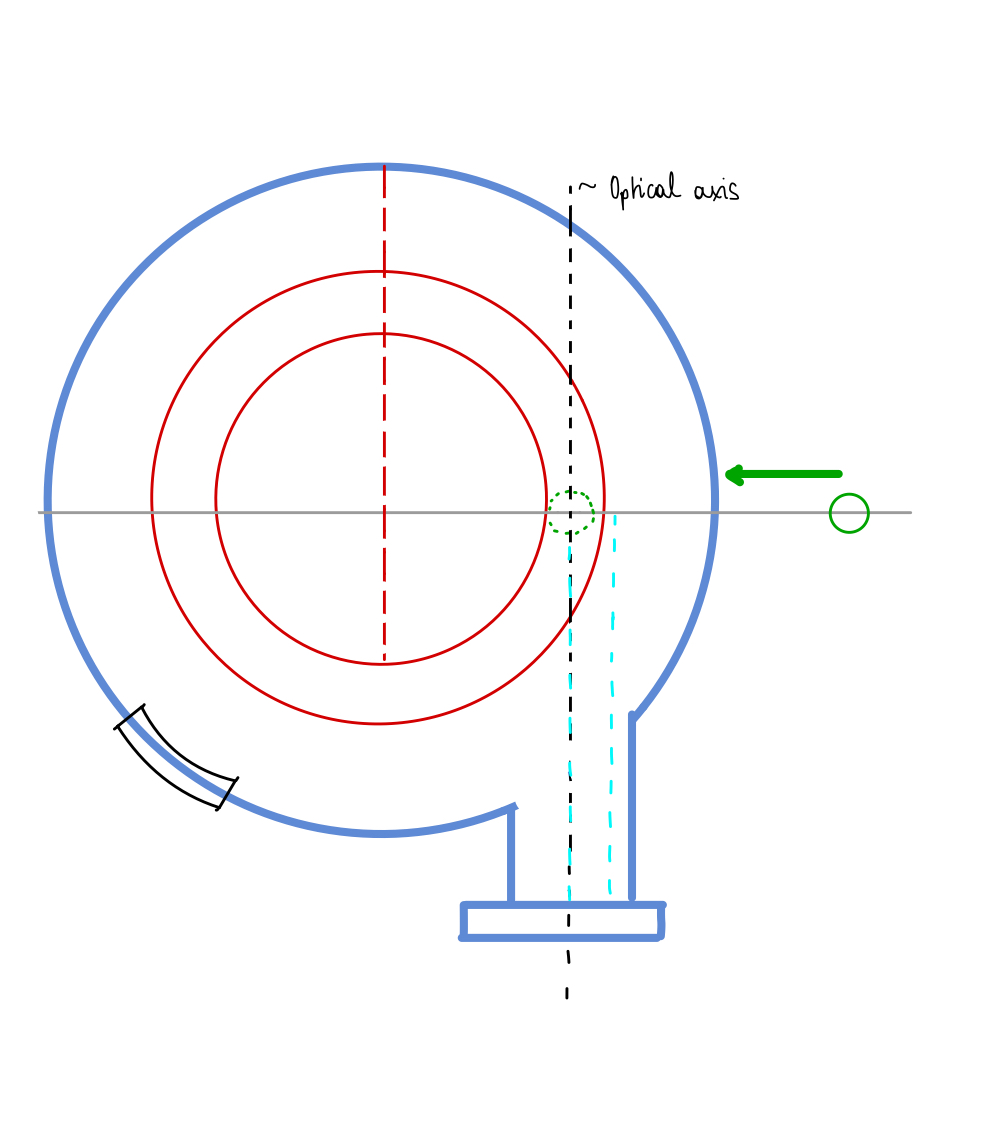
\includegraphics[width=0.4\textwidth]{sections/imges/ports/Flurescent_rod_new_sketch.jpeg}
        \subcaption{Sketch of the fluorescent rod and the window.}
        \label{fig:fluorescent_rod_sketch}
    \end{subfigure}
    \caption{Fluorescent rod.}
\end{figure}


Port 2 is the window, which is shown in the sketch \autoref{fig:fluorescent_rod}.
The window should be positioned in a way that the surface of the rod is parallel to ones line of sight.
For observation purpose, it is preferable to use quartz glass.
The desired size of the window should be as large as possible, with the minimum size being determined by the inclusion of the outermost closed flux surfaces in the projection.

Port 3 is the \emph{Langmuir probe}, its purpose is to measure the electron temperature, density and the electric potential of the plasma.
The location of the probe should be on the outside of the cylinder and points towards the center of the cylinder.
The size of the flange is as large as the maximum of the plasma cross-section plus $\approx 4~\si{\centi\meter}$.
To ensure the scanning of the entire plasma cross-section, the Langmuir probe needs to be movable in two directions.
Therefore an external vacuum vessel will be utilized to house the moving components of the probe.
The diameter of the probe will be $\SI{10}{\milli\meter}$ and its measuring tip $\SI{1}{\milli\meter}$.

Port 4 includes the \emph{Interferometer}.
It need to include 2 horn antennas from the outside and a mirror on the inside, which can be adjusted in the xy-plane.
The mirror need to be adjustable in the xy-plane in order to correct for the correct angle of the interferometer.
To move the mirror inside of the chamber a motor is required.
A sketch of the setup is shown in \autoref{fig:interferometer_setup}.
The horn antenna used in the interferometer is shown in \autoref{fig:horn_antena_interferometer}.
Also there specific size is given.

\begin{figure}[H]
    \centering
    \begin{subfigure}{0.4\textwidth}
        \centering
        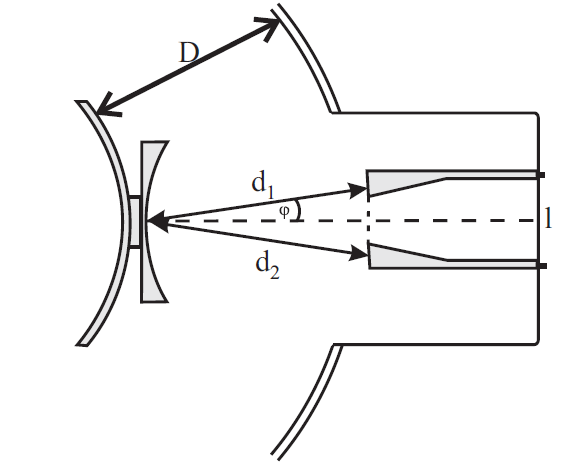
\includegraphics[width=1\textwidth]{sections/imges/ports/interferometer.png}
        \subcaption{Interferometer setup.}
        \label{fig:interferometer_setup}
    \end{subfigure}
    \hfill
    \begin{subfigure}{0.59\textwidth}
        \centering
        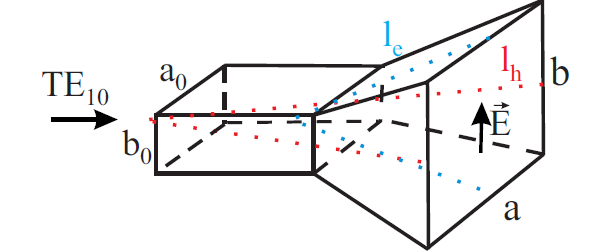
\includegraphics[width=1\textwidth]{sections/imges/ports/interferometer_horn_antena.png}
        \subcaption{Horn antenna used in the interferometer. With $a \approx (20 - 30)~\si{\milli\meter}$, $b \approx (16 - 22)~\si{\milli\meter}$ and  $l_e = l_h \approx 60~\si{\milli\meter}$ being the horn antenna. And $a_0^{\text{innen}} = 3.76~\si{\milli\meter}$, $a_0^{\text{außen}} = 5.79~\si{\milli\meter}$, $b_0^{\text{innen}} = 1.88~\si{\milli\meter}$, $b_0^{\text{außen}} = 3.91~\si{\milli\meter}$ being the waveguide WR-15 used by the TJ-K.}
        \label{fig:horn_antena_interferometer}
    \end{subfigure}
    \caption{Interferometer.}
    \label{fig:interferometer}
\end{figure}


Port 7 to 9 are the \emph{Rogowski coil} and the \emph{diamagnetic loops}.
The three measurement tools need each one a coaxial cable feedthrough connections.
For this a \textbf{KF-25} should be used, which is shown in \autoref{fig:coaxial_cable_feedthrough}.
The Rogowski coil and the two diamagnetic loops are spaced equally around the chamber and thus the cylindrical chamber.
Therefore, a distance of $\approx 120~\si{\degree}$ is chosen between the three ports.
The feedthrough are placed on the outside next to the coil and the loops, respectively.
A sketch of the setup is shown in \autoref{fig:rogowski_coil_diamagnetic_loops}.

\begin{figure}[H]
    \centering
    \begin{subfigure}{0.49\textwidth}
        \centering
        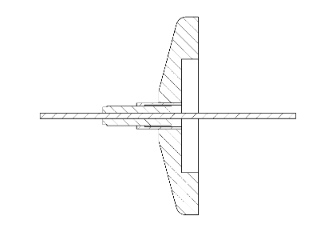
\includegraphics[width=1\textwidth]{sections/imges/ports/coaxial_feedthough.png}
        \subcaption{BNC coaxial throughput with KF-25 flange}
        \label{fig:coaxial_cable_feedthrough}
    \end{subfigure}
    \hfill
    \begin{subfigure}{0.49\textwidth}
        \centering
        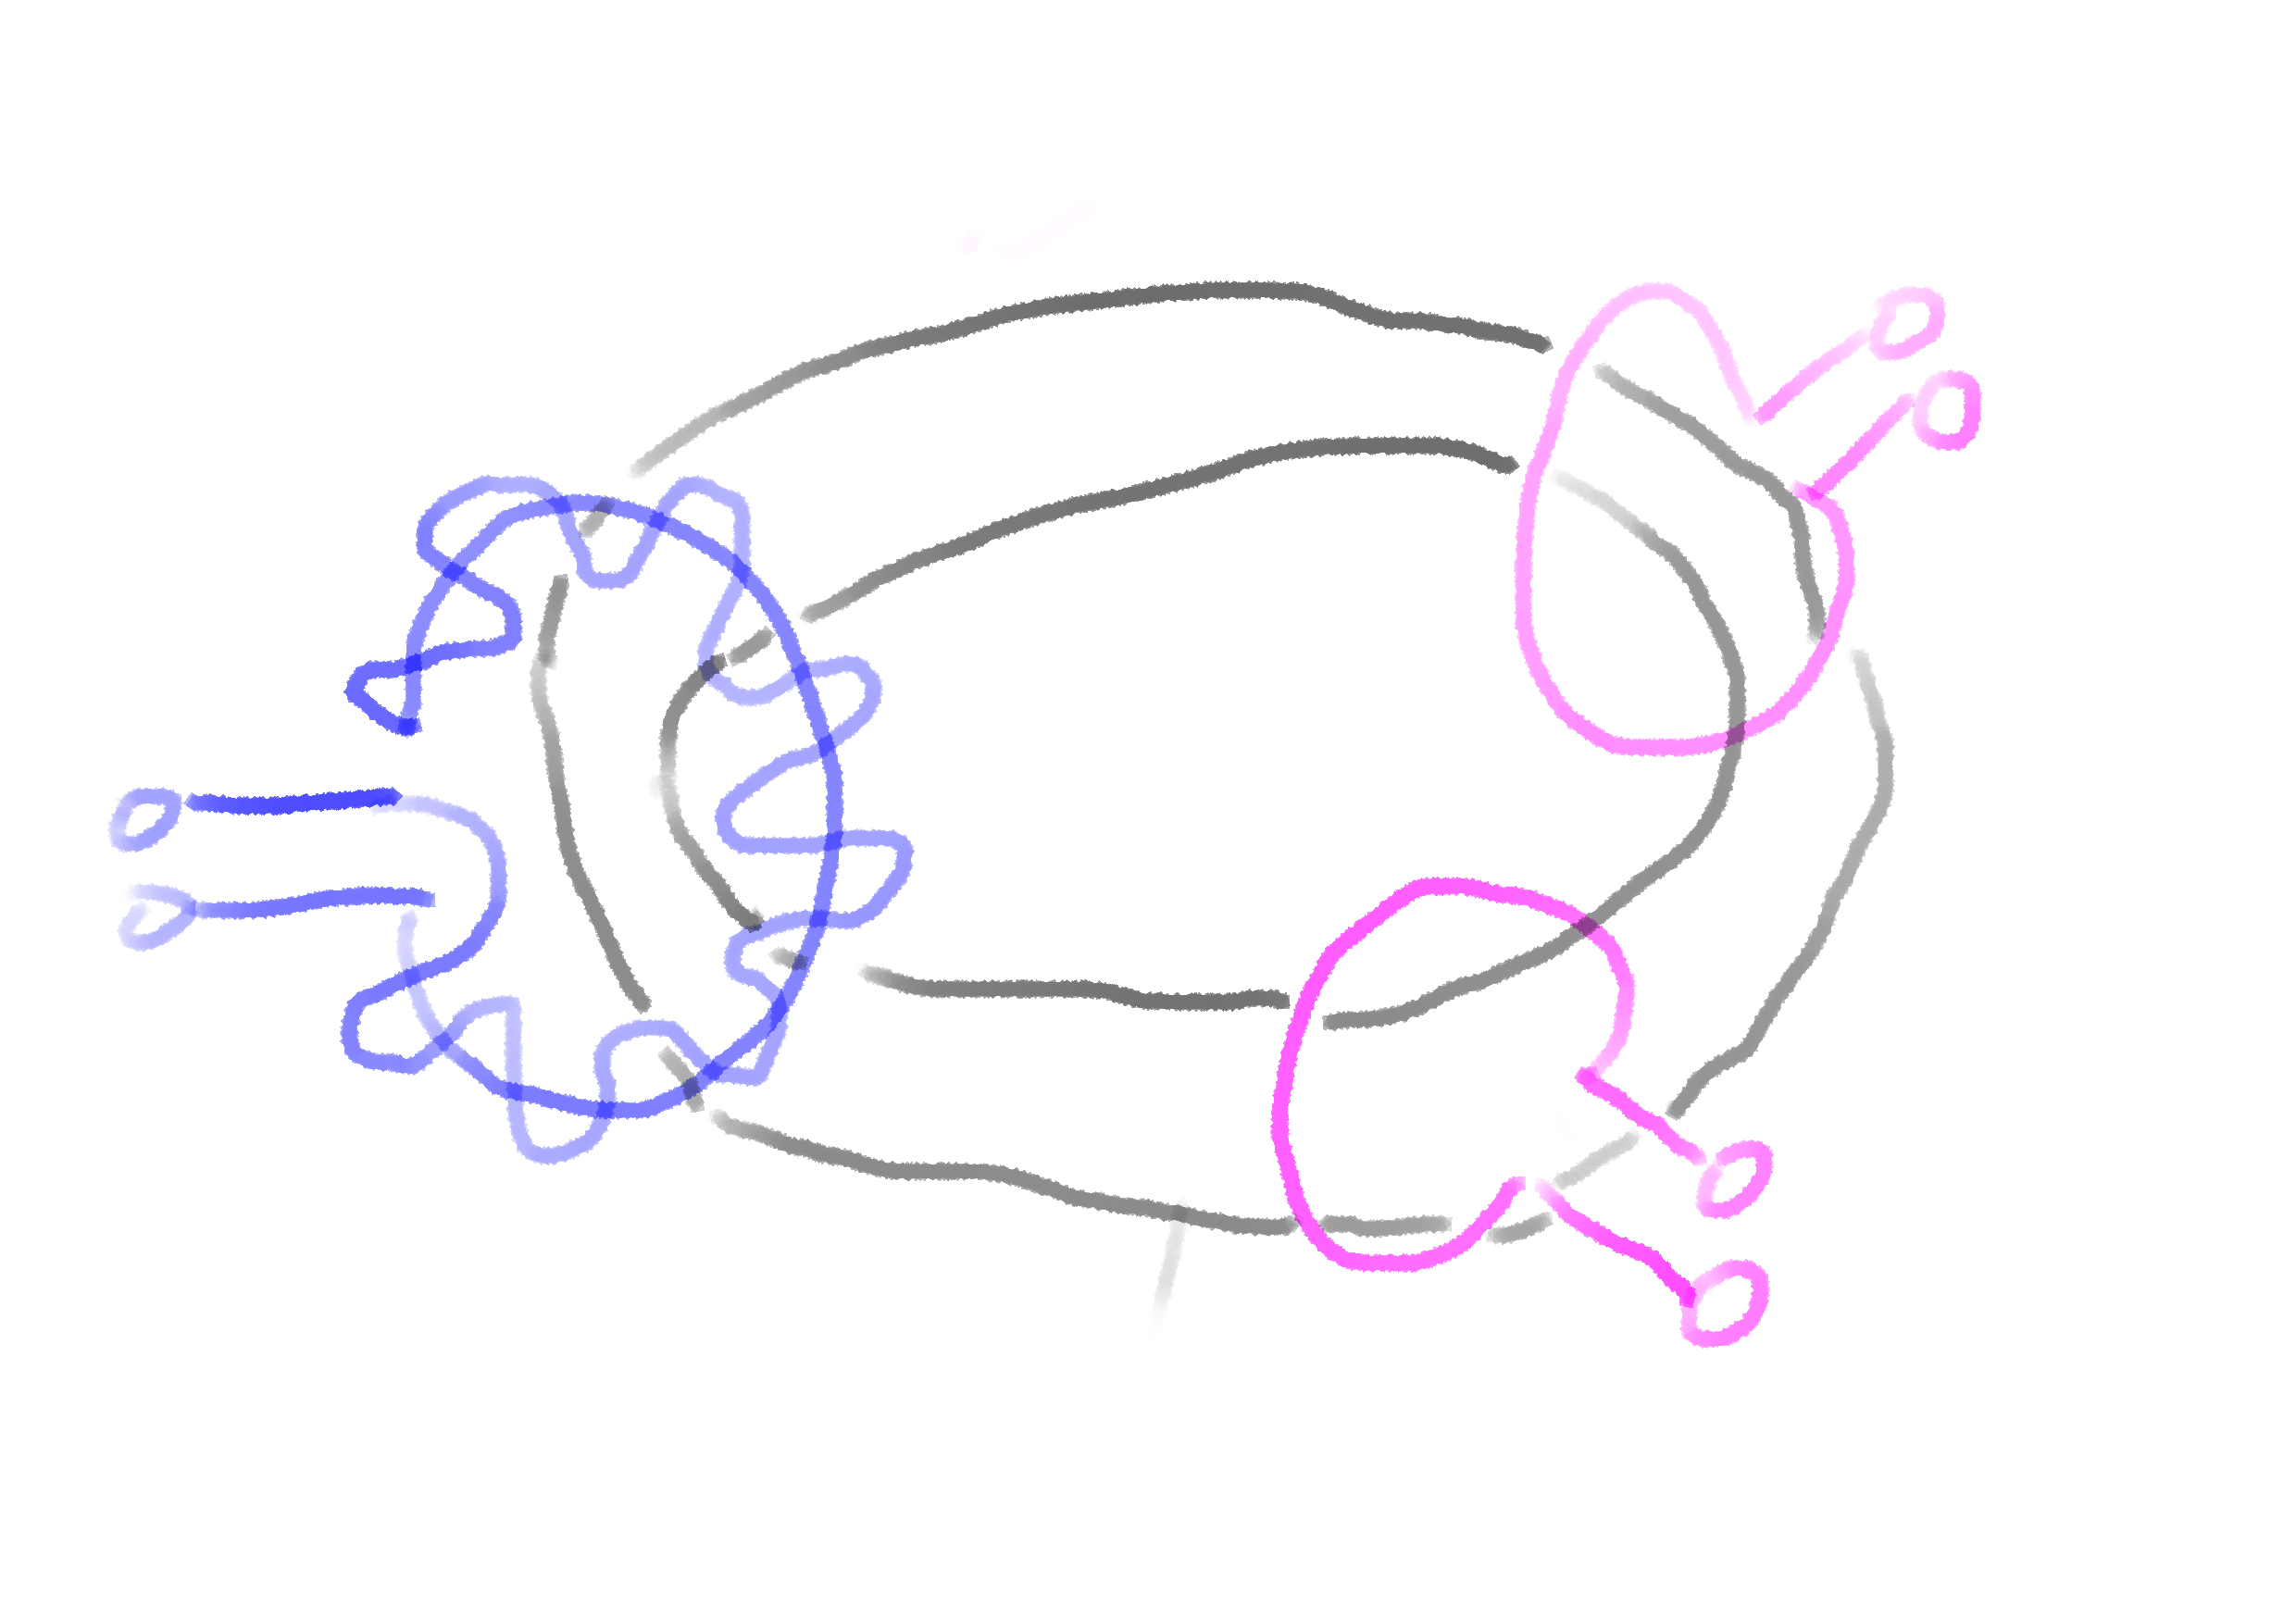
\includegraphics[width=1\textwidth]{sections/imges/ports/rogowski_coil_diamagnetx_loop.png}
        \subcaption{Sketch of the coil configuration around the toroidal plasma (black). The rogowski coil (blue) encloses an angle of $120\si{\degree}$ with each of the diamagnetic loops (pink). The wires leave the chamber by a coaxial troughput each.
        }
        \label{fig:rogowski_coil_diamagnetic_loops}
    \end{subfigure}
    \caption{Rogowski coil and diamagnetic loops with feedthrough.}
\end{figure}




\subsection{Heating - Team}
%\begin{table}[H]
    \centering
    \caption{Overview of the ports from the \textbf{heating team}.}
    \begin{tabular}{>{\raggedright\arraybackslash}p{2cm} >{\raggedright\arraybackslash}p{3cm} >{\raggedright\arraybackslash}p{3.5cm} >{\raggedright\arraybackslash}p{3.5cm} >{\raggedright\arraybackslash}p{2cm}}
        \toprule
        \textbf{Port} & \textbf{Purpose} & \textbf{Location} & \textbf{Type} & \textbf{Flange/Size} \\
        \midrule
        Port 1        &                  &                   &               &                      \\
        Port 2        &                  &                   &               &                      \\
        Port 3        &                  &                   &               &                      \\
        \bottomrule
    \end{tabular}
\end{table}

Unfortunately we did not got exact specifications nor exact definitions of their ports or locations.



\section{Conclusion}

As mentioned in the \autoref{sec:main_recipient} the process steps of the design of the main vacuum vessel is described.
The first idea was to use a simple cylindrical chamber with a flat lid and base.
This most simple design unfortunately did not fulfill the requirements of the vacuum chamber, as under the pressure difference of $\SI{e-9}{\milli\bar}$ to atmospheric pressure, the steel lid and base would band to much.
This made this design not feasible.

The second attempt was to use a supported base and a dome shaped lid.
With this the bottom can be designed much more rigid and be placed easily on a palette, which has some advantages concerning transportation.
The lid was designed dome shaped, which increased the rigidity a lot without increasing the thickness of the steel.
This is shown in \autoref{fig:Kekskochtopf_all} and \autoref{fig:Dose_all} for a flat and the dome shaped lid respectively.

The design of the vacuum chamber, which was finalized, is shown in \autoref{fig:Kammer_all}.
It has a dome shaped lid as well as a dome shaped base.
This allowed to increase the size of the chamber as the base and the lid are both removable and can be placed together inside a laboratory.
The given specifications of the size were given, that the chamber need to fit through a standard door, with the size of $\SI{90}{\centi\meter}$ times $\SI{200}{\centi\meter}$.

For the sake of simplicity, the same size was chosen for all connections except for the flange for the Pirani-Bayard-Alpert pressure measurement and the one for the quadrupole spectrometer, as little previous knowledge of specific flange sizes was known.
The size chosen was that of the TMP flange (see above), which has the advantage that the pump can in principle be fitted anywhere with the aid of a so-called knee.
Adapters can then be installed for all other connections to ensure that any other flange size can be connected.

Apart from the ports already known for the chamber, additional ports with standard flanges are added.
This makes is easier for the future use of the chamber, as retrofitting extra ports is not necessary.
Also adding ports from the beginning makes it cheaper, as not much work is needed to add them later on.


\section{Outlook}

The vacuum chamber must be robust enough to withstand the pressure difference between its interior and exterior, and it must also be versatile enough to accommodate various ports and feedthroughs for different purposes.
As we move forward, the design of the vacuum chamber may need to be adjusted based on the specific requirements of the other teams involved in the design process.
The exact number and types of ports, as well as other components such as windows, gas inlets, feedthroughs, and coaxials, have not been finalized yet.
Therefore, additional work will be needed to finalize these details and to ensure that the vacuum chamber design meets all necessary requirements.
At this stage, the cost of the vacuum chamber itself remains unknown and cannot be estimated.
The manufacturer does not provide list prices for such custom-made items and would only provide a cost estimate upon specific order inquiry.
It is anticipated that the vacuum chamber itself would represent one of the largest expenses for the entire project, primarily due to the necessity of custom manufacturing.
